\section{Результаты измерений}
\begin{table}[!ht]
    \centering
    \begin{tabular}{|l|l|l|}
    \hline
        $T,\pm 0.05\;\text{К}$ & $h_1,\pm 0.0025\;\text{см}$ & $h_2,\pm 0.0025\;\text{см}$ \\ \hline
        293 & 5.19 & 2.58 \\ \hline
        295 & 5.3 & 2.5 \\ \hline
        296 & 5.345 & 2.44 \\ \hline
        297 & 5.42 & 2.36 \\ \hline
        298 & 5.5 & 2.295 \\ \hline
        299 & 5.55 & 2.34 \\ \hline
        300 & 5.645 & 2.185 \\ \hline
        301 & 5.71 & 2.11 \\ \hline
        302 & 5.695 & 2.02 \\ \hline
        303 & 5.88 & 1.955 \\ \hline
        304 & 5.94 & 1.88 \\ \hline
        305 & 6.02 & 1.81 \\ \hline
        306 & 6.135 & 1.69 \\ \hline
        307 & 6.27 & 1.565 \\ \hline
        308 & 6.38 & 1.47 \\ \hline
        309 & 6.49 & 1.355 \\ \hline
        310 & 6.61 & 1.24 \\ \hline
        311 & 6.74 & 1.1 \\ \hline
        312 & 6.89 & 1 \\ \hline
        313 & 7.07 & 0.83 \\ \hline
        310.93 & 6.81 & 1.05 \\ \hline
        310.03 & 6.705 & 1.19 \\ \hline
        309.04 & 6.62 & 1.295 \\ \hline
        308 & 6.49 & 1.42 \\ \hline
        307.04 & 6.38 & 1.525 \\ \hline
        305.98 & 6.26 & 1.64 \\ \hline
        305.05 & 6.16 & 1.7 \\ \hline
        303.98 & 6.06 & 1.82 \\ \hline
        303.02 & 5.95 & 1.89 \\ \hline
        302.02 & 5.885 & 1.98 \\ \hline
        301.04 & 5.795 & 2.06 \\ \hline
        300.03 & 5.705 & 2.16 \\ \hline
        299.03 & 5.65 & 2.21 \\ \hline
        298.03 & 5.55 & 2.27 \\ \hline
        297.03 & 5.47 & 2.34 \\ \hline
        296.04 & 5.41 & 2.4 \\ \hline
        295.05 & 5.34 & 2.455 \\ \hline
        294.03 & 5.28 & 2.53 \\ \hline
        293.05 & 5.22 & 2.58 \\ \hline
    \end{tabular}
\end{table}

$h_2$ --- высота столба ртути в трубке, соедененной с запаянной жидкостью, $h_1$ ---
высота столба ртути в другой трубке. Над трубкой, примыкающей к сосуду с жидкостью,
образовался водяной столб высотой $\Delta h = 8{,}4\pm 0{,}0025\;\text{см}$, который надо учитывать.

Плотность ртути из таблицы $\rho_\text{Hg}=13550\;\text{кг}/\text{м}^3$, воды $rho=1000\;\text{кг}/\text{м}^3$.
Давление в сосуде находим по формуле
\[P=\rho_\text{Hg}g(h_2-h_2)-\rho g\Delta h\]

Строим графики и находим их наклоны:
\begin{center}
    $k_1 = 232\pm 6\;\text{Па}/\text{К}$\\
    $k_2 = -4710\pm 60\;\text{К}$
\end{center}

Тогда теплоты испарения:
\begin{center}
    $L_1 = \frac{R\overline{T}^2}{\overline{P}}k_1 = 38\pm 1\;\text{Дж}/\text{моль}$\\
    $L_2 = -Rk_2 = 39{,}1\pm 0{,}5\;\;\text{Дж}/\text{моль}$
\end{center}

$\overline{T}$ --- среднее значение температуры, $\overline{P}$ --- среднее значение давления
за время проведения эксперимента.

\begin{figure}[ht!]
    \centering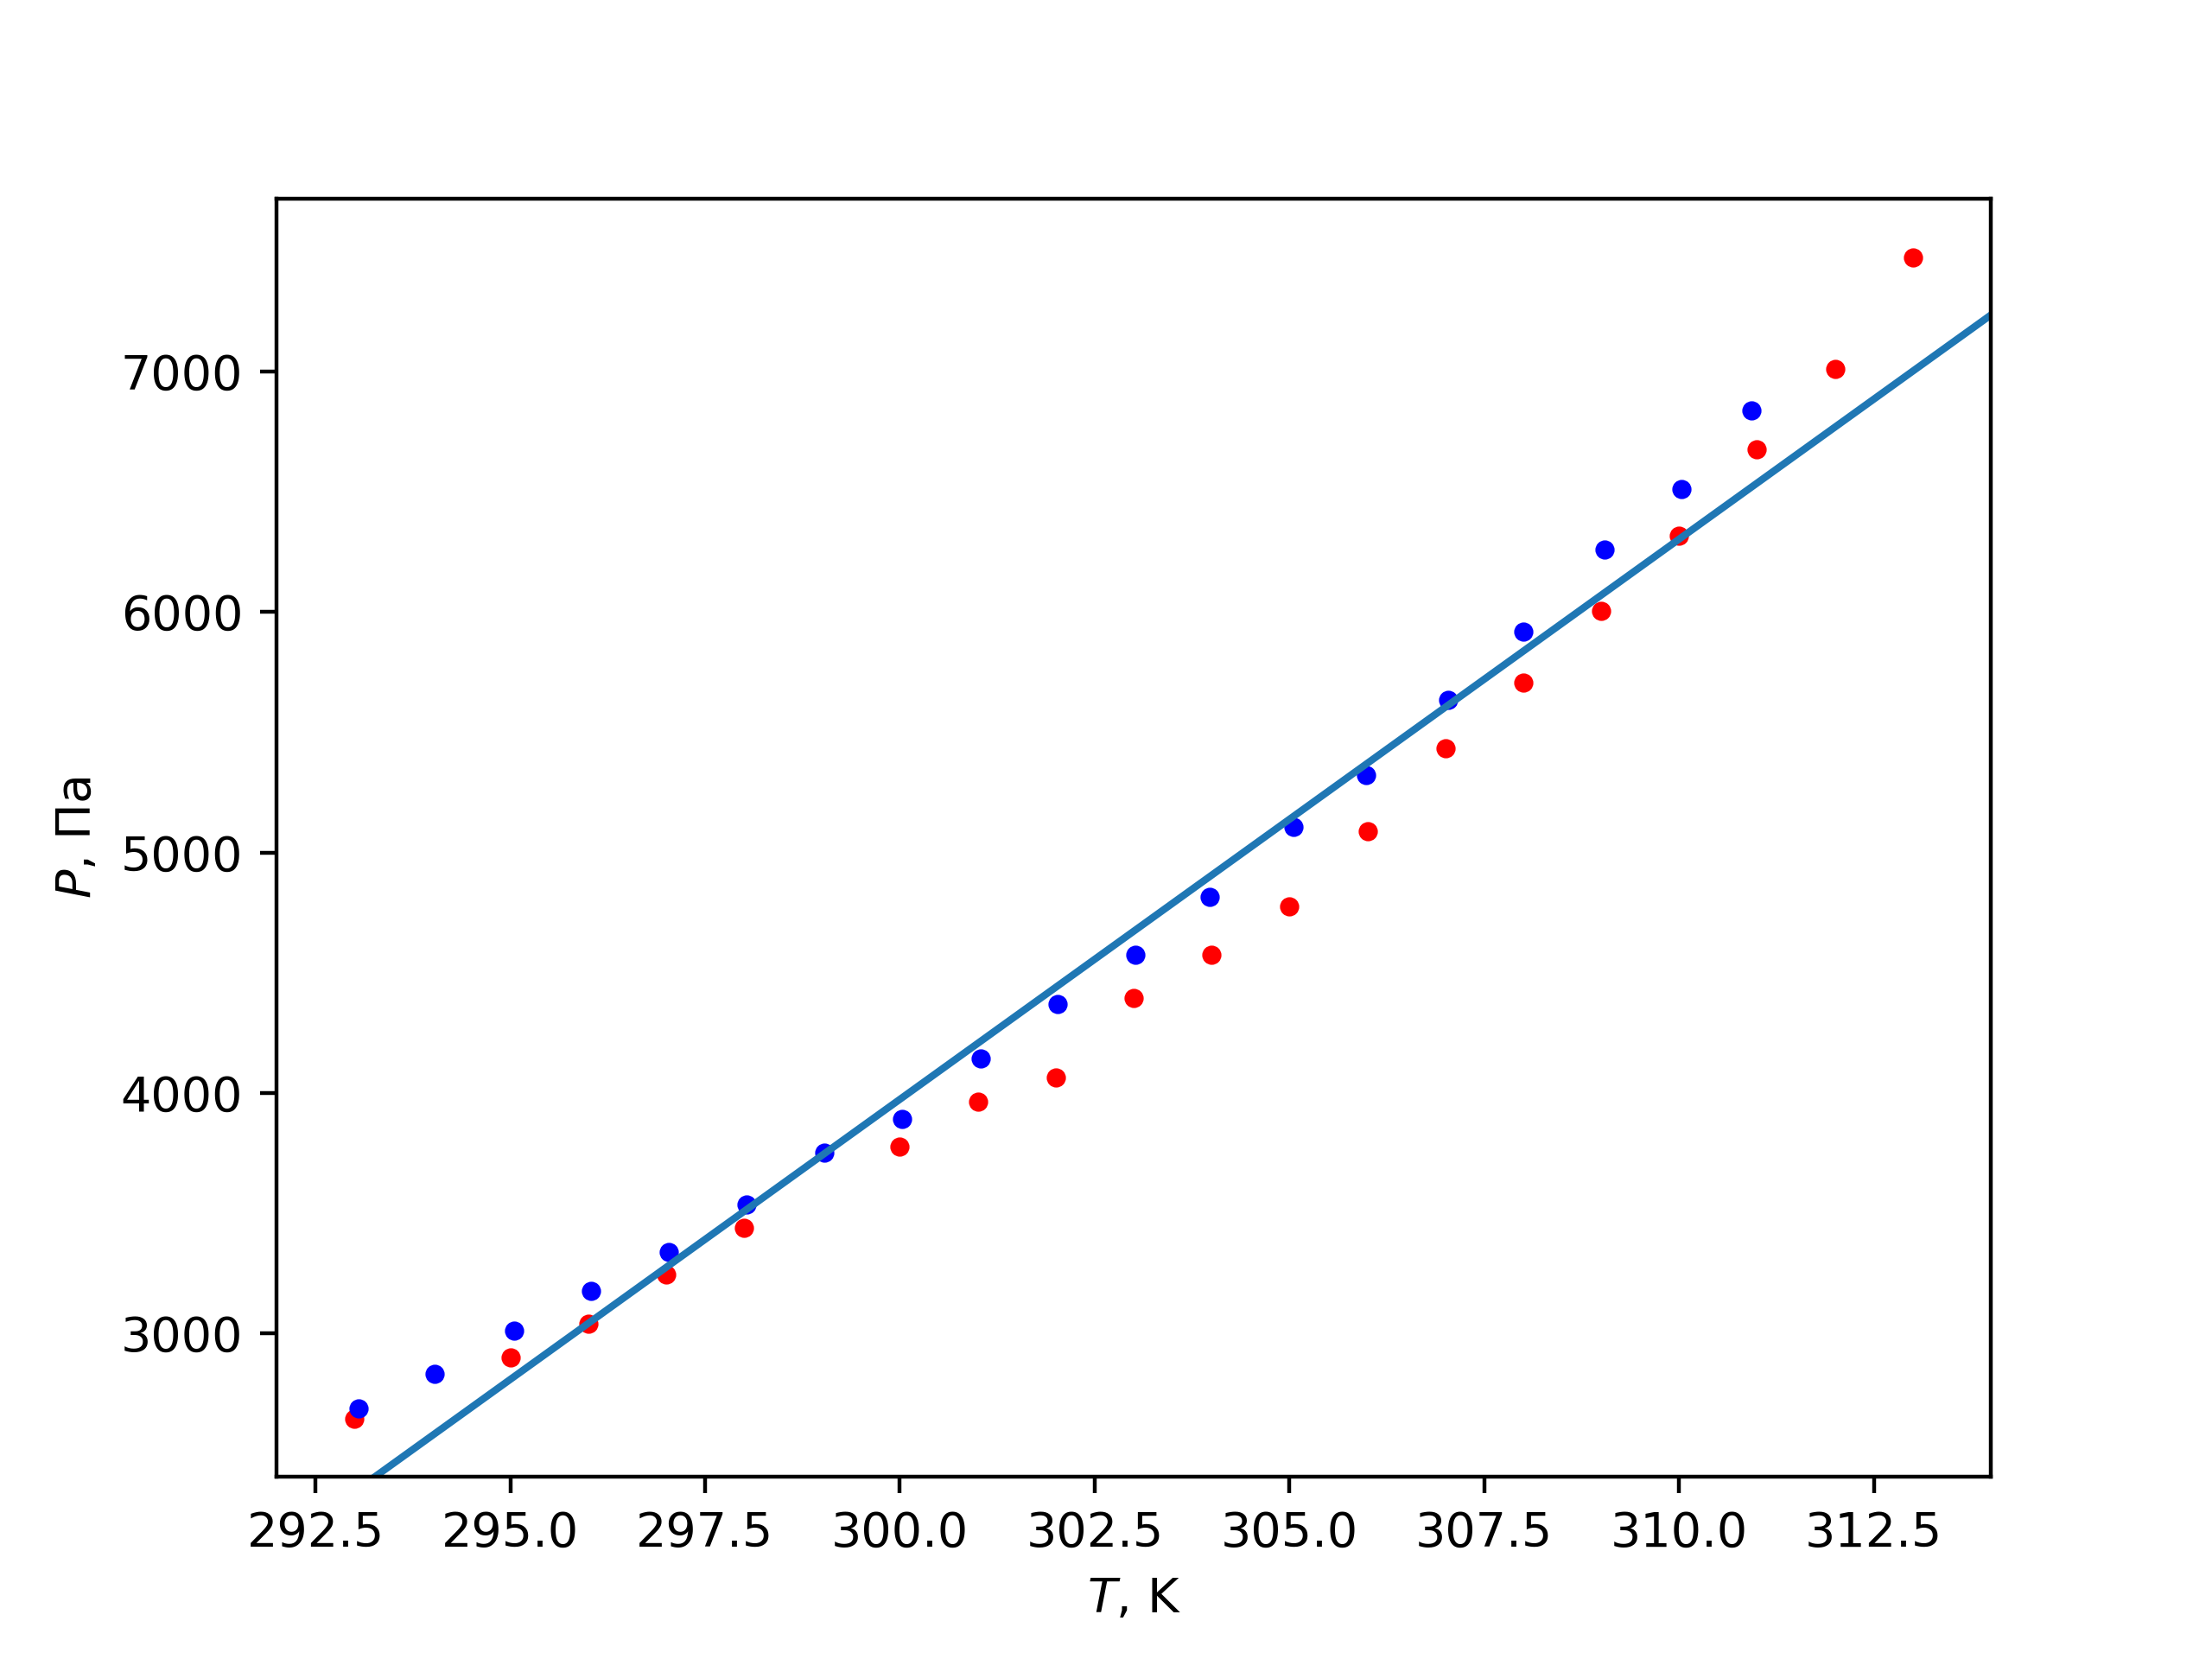
\includegraphics[width=0.8\linewidth]{img/plot1}
\end{figure}
\begin{figure}[ht!]
    \centering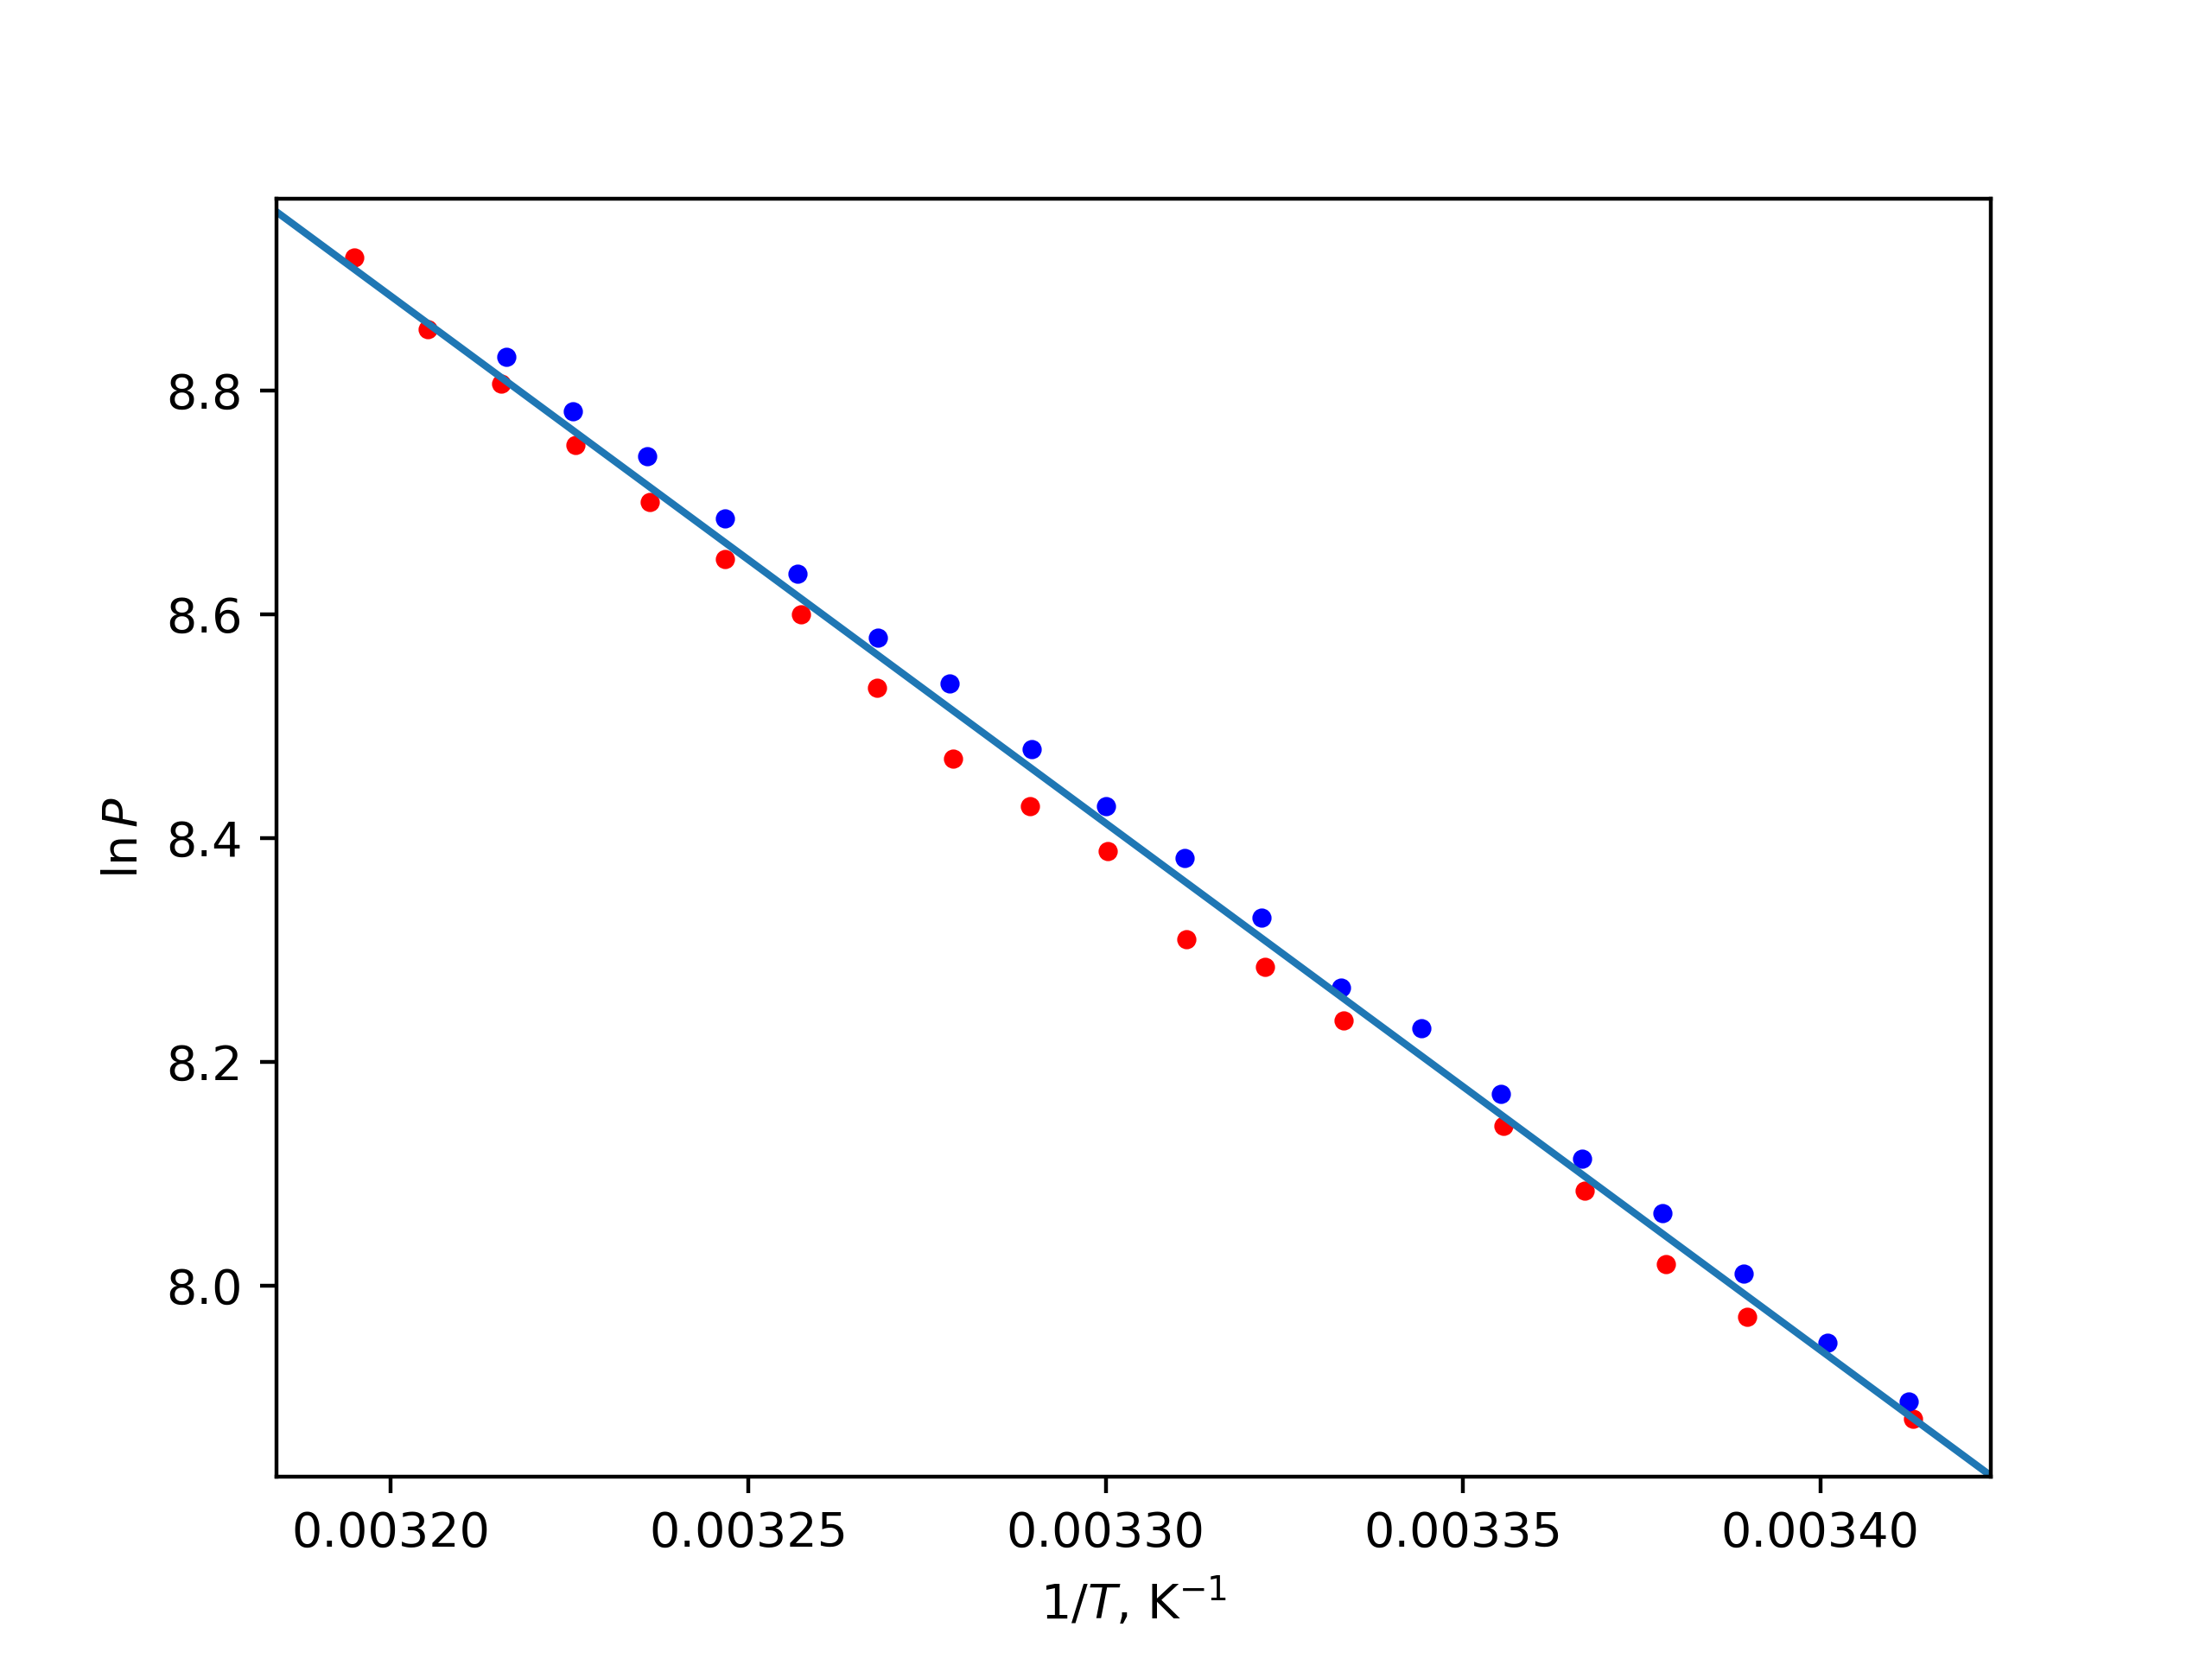
\includegraphics[width=0.8\linewidth]{img/plot2}
\end{figure}
